%% bare_conf.tex
%% V1.4a
%% 2014/09/17
%% by Michael Shell
%% See:
%% http://www.michaelshell.org/
%% for current contact information.
%%
%% This is a skeleton file demonstrating the use of IEEEtran.cls
%% (requires IEEEtran.cls version 1.8a or later) with an IEEE
%% conference paper.
%%
%% Support sites:
%% http://www.michaelshell.org/tex/ieeetran/
%% http://www.ctan.org/tex-archive/macros/latex/contrib/IEEEtran/
%% and
%% http://www.ieee.org/

%%*************************************************************************
%% Legal Notice:
%% This code is offered as-is without any warranty either expressed or
%% implied; without even the implied warranty of MERCHANTABILITY or
%% FITNESS FOR A PARTICULAR PURPOSE! 
%% User assumes all risk.
%% In no event shall IEEE or any contributor to this code be liable for
%% any damages or losses, including, but not limited to, incidental,
%% consequential, or any other damages, resulting from the use or misuse
%% of any information contained here.
%%
%% All comments are the opinions of their respective authors and are not
%% necessarily endorsed by the IEEE.
%%
%% This work is distributed under the LaTeX Project Public License (LPPL)
%% ( http://www.latex-project.org/ ) version 1.3, and may be freely used,
%% distributed and modified. A copy of the LPPL, version 1.3, is included
%% in the base LaTeX documentation of all distributions of LaTeX released
%% 2003/12/01 or later.
%% Retain all contribution notices and credits.
%% ** Modified files should be clearly indicated as such, including  **
%% ** renaming them and changing author support contact information. **
%%
%% File list of work: IEEEtran.cls, IEEEtran_HOWTO.pdf, bare_adv.tex,
%%                    bare_conf.tex, bare_jrnl.tex, bare_conf_compsoc.tex,
%%                    bare_jrnl_compsoc.tex, bare_jrnl_transmag.tex
%%*************************************************************************


% *** Authors should verify (and, if needed, correct) their LaTeX system  ***
% *** with the testflow diagnostic prior to trusting their LaTeX platform ***
% *** with production work. IEEE's font choices and paper sizes can       ***
% *** trigger bugs that do not appear when using other class files.       ***                          ***
% The testflow support page is at:
% http://www.michaelshell.org/tex/testflow/



\documentclass[conference, 11pt]{IEEEtran}
% Some Computer Society conferences also require the compsoc mode option,
% but others use the standard conference format.
%
% If IEEEtran.cls has not been installed into the LaTeX system files,
% manually specify the path to it like:
% \documentclass[conference]{../sty/IEEEtran}



% Some very useful LaTeX packages include:
% (uncomment the ones you want to load)


% *** MISC UTILITY PACKAGES ***
%
%\usepackage{ifpdf}
% Heiko Oberdiek's ifpdf.sty is very useful if you need conditional
% compilation based on whether the output is pdf or dvi.
% usage:
% \ifpdf
%   % pdf code
% \else
%   % dvi code
% \fi
% The latest version of ifpdf.sty can be obtained from:
% http://www.ctan.org/tex-archive/macros/latex/contrib/oberdiek/
% Also, note that IEEEtran.cls V1.7 and later provides a builtin
% \ifCLASSINFOpdf conditional that works the same way.
% When switching from latex to pdflatex and vice-versa, the compiler may
% have to be run twice to clear warning/error messages.






% *** CITATION PACKAGES ***
%
%\usepackage{cite}
% cite.sty was written by Donald Arseneau
% V1.6 and later of IEEEtran pre-defines the format of the cite.sty package
% \cite{} output to follow that of IEEE. Loading the cite package will
% result in citation numbers being automatically sorted and properly
% "compressed/ranged". e.g., [1], [9], [2], [7], [5], [6] without using
% cite.sty will become [1], [2], [5]--[7], [9] using cite.sty. cite.sty's
% \cite will automatically add leading space, if needed. Use cite.sty's
% noadjust option (cite.sty V3.8 and later) if you want to turn this off
% such as if a citation ever needs to be enclosed in parenthesis.
% cite.sty is already installed on most LaTeX systems. Be sure and use
% version 5.0 (2009-03-20) and later if using hyperref.sty.
% The latest version can be obtained at:
% http://www.ctan.org/tex-archive/macros/latex/contrib/cite/
% The documentation is contained in the cite.sty file itself.






% *** GRAPHICS RELATED PACKAGES ***
%
\ifCLASSINFOpdf
  % \usepackage[pdftex]{graphicx}
  % declare the path(s) where your graphic files are
  % \graphicspath{{../pdf/}{../jpeg/}}
  % and their extensions so you won't have to specify these with
  % every instance of \includegraphics
  % \DeclareGraphicsExtensions{.pdf,.jpeg,.png}
\else
  % or other class option (dvipsone, dvipdf, if not using dvips). graphicx
  % will default to the driver specified in the system graphics.cfg if no
  % driver is specified.
  % \usepackage[dvips]{graphicx}
  % declare the path(s) where your graphic files are
  % \graphicspath{{../eps/}}
  % and their extensions so you won't have to specify these with
  % every instance of \includegraphics
  % \DeclareGraphicsExtensions{.eps}
\fi
% graphicx was written by David Carlisle and Sebastian Rahtz. It is
% required if you want graphics, photos, etc. graphicx.sty is already
% installed on most LaTeX systems. The latest version and documentation
% can be obtained at: 
% http://www.ctan.org/tex-archive/macros/latex/required/graphics/
% Another good source of documentation is "Using Imported Graphics in
% LaTeX2e" by Keith Reckdahl which can be found at:
% http://www.ctan.org/tex-archive/info/epslatex/
%
% latex, and pdflatex in dvi mode, support graphics in encapsulated
% postscript (.eps) format. pdflatex in pdf mode supports graphics
% in .pdf, .jpeg, .png and .mps (metapost) formats. Users should ensure
% that all non-photo figures use a vector format (.eps, .pdf, .mps) and
% not a bitmapped formats (.jpeg, .png). IEEE frowns on bitmapped formats
% which can result in "jaggedy"/blurry rendering of lines and letters as
% well as large increases in file sizes.
%
% You can find documentation about the pdfTeX application at:
% http://www.tug.org/applications/pdftex





% *** MATH PACKAGES ***
%
%\usepackage[cmex10]{amsmath}
% A popular package from the American Mathematical Society that provides
% many useful and powerful commands for dealing with mathematics. If using
% it, be sure to load this package with the cmex10 option to ensure that
% only type 1 fonts will utilized at all point sizes. Without this option,
% it is possible that some math symbols, particularly those within
% footnotes, will be rendered in bitmap form which will result in a
% document that can not be IEEE Xplore compliant!
%
% Also, note that the amsmath package sets \interdisplaylinepenalty to 10000
% thus preventing page breaks from occurring within multiline equations. Use:
%\interdisplaylinepenalty=2500
% after loading amsmath to restore such page breaks as IEEEtran.cls normally
% does. amsmath.sty is already installed on most LaTeX systems. The latest
% version and documentation can be obtained at:
% http://www.ctan.org/tex-archive/macros/latex/required/amslatex/math/





% *** SPECIALIZED LIST PACKAGES ***
%
%\usepackage{algorithmic}
% algorithmic.sty was written by Peter Williams and Rogerio Brito.
% This package provides an algorithmic environment fo describing algorithms.
% You can use the algorithmic environment in-text or within a figure
% environment to provide for a floating algorithm. Do NOT use the algorithm
% floating environment provided by algorithm.sty (by the same authors) or
% algorithm2e.sty (by Christophe Fiorio) as IEEE does not use dedicated
% algorithm float types and packages that provide these will not provide
% correct IEEE style captions. The latest version and documentation of
% algorithmic.sty can be obtained at:
% http://www.ctan.org/tex-archive/macros/latex/contrib/algorithms/
% There is also a support site at:
% http://algorithms.berlios.de/index.html
% Also of interest may be the (relatively newer and more customizable)
% algorithmicx.sty package by Szasz Janos:
% http://www.ctan.org/tex-archive/macros/latex/contrib/algorithmicx/




% *** ALIGNMENT PACKAGES ***
%
%\usepackage{array}
% Frank Mittelbach's and David Carlisle's array.sty patches and improves
% the standard LaTeX2e array and tabular environments to provide better
% appearance and additional user controls. As the default LaTeX2e table
% generation code is lacking to the point of almost being broken with
% respect to the quality of the end results, all users are strongly
% advised to use an enhanced (at the very least that provided by array.sty)
% set of table tools. array.sty is already installed on most systems. The
% latest version and documentation can be obtained at:
% http://www.ctan.org/tex-archive/macros/latex/required/tools/


% IEEEtran contains the IEEEeqnarray family of commands that can be used to
% generate multiline equations as well as matrices, tables, etc., of high
% quality.




% *** SUBFIGURE PACKAGES ***
%\ifCLASSOPTIONcompsoc
%  \usepackage[caption=false,font=normalsize,labelfont=sf,textfont=sf]{subfig}
%\else
%  \usepackage[caption=false,font=footnotesize]{subfig}
%\fi
% subfig.sty, written by Steven Douglas Cochran, is the modern replacement
% for subfigure.sty, the latter of which is no longer maintained and is
% incompatible with some LaTeX packages including fixltx2e. However,
% subfig.sty requires and automatically loads Axel Sommerfeldt's caption.sty
% which will override IEEEtran.cls' handling of captions and this will result
% in non-IEEE style figure/table captions. To prevent this problem, be sure
% and invoke subfig.sty's "caption=false" package option (available since
% subfig.sty version 1.3, 2005/06/28) as this is will preserve IEEEtran.cls
% handling of captions.
% Note that the Computer Society format requires a larger sans serif font
% than the serif footnote size font used in traditional IEEE formatting
% and thus the need to invoke different subfig.sty package options depending
% on whether compsoc mode has been enabled.
%
% The latest version and documentation of subfig.sty can be obtained at:
% http://www.ctan.org/tex-archive/macros/latex/contrib/subfig/




% *** FLOAT PACKAGES ***
%
%\usepackage{fixltx2e}
% fixltx2e, the successor to the earlier fix2col.sty, was written by
% Frank Mittelbach and David Carlisle. This package corrects a few problems
% in the LaTeX2e kernel, the most notable of which is that in current
% LaTeX2e releases, the ordering of single and double column floats is not
% guaranteed to be preserved. Thus, an unpatched LaTeX2e can allow a
% single column figure to be placed prior to an earlier double column
% figure. The latest version and documentation can be found at:
% http://www.ctan.org/tex-archive/macros/latex/base/


%\usepackage{stfloats}
% stfloats.sty was written by Sigitas Tolusis. This package gives LaTeX2e
% the ability to do double column floats at the bottom of the page as well
% as the top. (e.g., "\begin{figure*}[!b]" is not normally possible in
% LaTeX2e). It also provides a command:
%\fnbelowfloat
% to enable the placement of footnotes below bottom floats (the standard
% LaTeX2e kernel puts them above bottom floats). This is an invasive package
% which rewrites many portions of the LaTeX2e float routines. It may not work
% with other packages that modify the LaTeX2e float routines. The latest
% version and documentation can be obtained at:
% http://www.ctan.org/tex-archive/macros/latex/contrib/sttools/
% Do not use the stfloats baselinefloat ability as IEEE does not allow
% \baselineskip to stretch. Authors submitting work to the IEEE should note
% that IEEE rarely uses double column equations and that authors should try
% to avoid such use. Do not be tempted to use the cuted.sty or midfloat.sty
% packages (also by Sigitas Tolusis) as IEEE does not format its papers in
% such ways.
% Do not attempt to use stfloats with fixltx2e as they are incompatible.
% Instead, use Morten Hogholm'a dblfloatfix which combines the features
% of both fixltx2e and stfloats:
%
% \usepackage{dblfloatfix}
% The latest version can be found at:
% http://www.ctan.org/tex-archive/macros/latex/contrib/dblfloatfix/


%% Language and font encodings
\usepackage[english, ngerman]{babel}
\usepackage[utf8x]{inputenc}
\usepackage[T1]{fontenc}

%% Sets page size and margins
\usepackage[a4paper,top=3cm,bottom=2cm,left=3cm,right=3cm,marginparwidth=1.75cm]{geometry}

%% Useful packages
\usepackage{amsmath}
\usepackage{graphicx}
\usepackage[colorinlistoftodos]{todonotes}
\usepackage{xpatch}
\usepackage[hyphens]{url}
\usepackage[colorlinks=true, allcolors=blue]{hyperref}

\usepackage{float}

% *** PDF, URL AND HYPERLINK PACKAGES ***
%
%\usepackage{url}
% url.sty was written by Donald Arseneau. It provides better support for
% handling and breaking URLs. url.sty is already installed on most LaTeX
% systems. The latest version and documentation can be obtained at:
% http://www.ctan.org/tex-archive/macros/latex/contrib/url/
% Basically, \url{my_url_here}.




% *** Do not adjust lengths that control margins, column widths, etc. ***
% *** Do not use packages that alter fonts (such as pslatex).         ***
% There should be no need to do such things with IEEEtran.cls V1.6 and later.
% (Unless specifically asked to do so by the journal or conference you plan
% to submit to, of course. )


% correct bad hyphenation here
\hyphenation{op-tical net-works semi-conduc-tor}



\begin{document}


%
% paper title
% Titles are generally capitalized except for words such as a, an, and, as,
% at, but, by, for, in, nor, of, on, or, the, to and up, which are usually
% not capitalized unless they are the first or last word of the title.
% Linebreaks \\ can be used within to get better formatting as desired.
% Do not put math or special symbols in the title.
\title{Virtuelle Bühnenbilder mit der HoloLens}


% author names and affiliations
% use a multiple column layout for up to three different
% affiliations
\author{
	\IEEEauthorblockN{Tobias Berthold}
	\IEEEauthorblockA{Hochschule Darmstadt\\
	Haardtring 100, 64295 Darmstadt\\
	Email: \href{tobias.berthold@stud.h-da.de}{\nolinkurl{tobias.berthold@stud.h-da.de}}}\\
	\IEEEauthorblockN{Kin Liu}
	\IEEEauthorblockA{Hochschule Darmstadt\\
		Haardtring 100, 64295 Darmstadt\\
		Email: \href{mailto:kin.liu@stud.h-da.de}{\nolinkurl{kin.liu@stud.h-da.de}}}

\and
	\IEEEauthorblockN{Peter Enenkel}
	\IEEEauthorblockA{Hochschule Darmstadt\\
		Haardtring 100, 64295 Darmstadt\\
		Email: \href{mailto:peter.enenkel@stud.h-da.de}{\nolinkurl{peter.enenkel@stud.h-da.de}}}\\
	\IEEEauthorblockN{Mario Miosga}
	\IEEEauthorblockA{Hochschule Darmstadt\\
		Haardtring 100, 64295 Darmstadt\\
		Email: \href{mailto:mario.miosga@stud.h-da.de}{\nolinkurl{mario.miosga@stud.h-da.de}}
	}
}

% use for special paper notices
%\IEEEspecialpapernotice{(Invited Paper)}

% force page number to title page 
\patchcmd{\titlepage}
  {\thispagestyle{empty}}
  {\thispagestyle{plain}}
  {}
  {}

% make the title area
\maketitle
\thispagestyle{plain}
\pagestyle{plain}

% As a general rule, do not put math, special symbols or citations
% in the abstract
%\begin{abstract}
%The abstract goes here.
%\end{abstract}

% no keywords




% For peer review papers, you can put extra information on the cover
% page as needed:
% \ifCLASSOPTIONpeerreview
% \begin{center} \bfseries EDICS Category: 3-BBND \end{center}
% \fi
%
% For peerreview papers, this IEEEtran command inserts a page break and
% creates the second title. It will be ignored for other modes.
\IEEEpeerreviewmaketitle




\section{Einführung}

In der Industrie wird virtuelle Produktentwicklung schon lange genutzt. Eine Adaption dieser Technik für die Theaterwelt würde einige Vorteile bieten.
Die Herstellung der teilweise riesigen Leinwände der Bühnenbilder ist aufwendig und teuer. Auf der realen Bühne finden häufig Proben statt. Licht- und Tontechnik, die Schauspieler und/oder Musiker müssen alle zeitlich miteinander koordiniert werden. Auch kann der Aufbau von einem zum anderen Stück nicht immer einfach bewerkstelligt werden. Mit einer Fertigstellung des Bühnenbilds als virtueller Prototyp auf der realen Bühne, könnte man beispielsweise die Wirkung vorher testen, ohne wie bisher auf reine Computersimulationen und physikalische Modelle zurückgreifen zu müssen. \par
Eine komplett virtuelle Simulation lässt die Einbindung der tatsächlichen Bühne und Schauspieler nicht zu. Mit Augmented/Mixed Reality, also der Kombination von Realität und virtuellen Elementen – wie bei der Microsoft HoloLens - hingegen, ist dies möglich. Auch sicherheitstechnisch ist die Verwendung von virtuellen Objekten auf einer Bühne, solange die Realität nicht komplett überdeckt wird, vorstellbar. Statt auf Displays schauen zu müssen, kann der Bediener die Maschinerie der Bühne jederzeit im Auge behalten und sich gleichzeitig holographisch Informationen dazu einblenden lassen. \par 
Im Wintersemester 2016/17 wurde im Fachbereich Informatik an der Hochschule Darmstadt ein Master Projektseminar in Zusammenarbeit und Unterstützung der Firma Bosch Rexroth AG mit dem Titel \glqq Virtuelle Bühnenbilder mit der HoloLens\grqq \, begonnen. Die Zielsetzung dieses Projektes war und ist es einen Prototyp zu entwickeln, der Augmented Reality in einer Theaterumgebung nutzbar macht. Das folgende Paper zeigt die Ergebnisse des Wintersemester 2016/17 dieses Projektes, die vornehmlich eine Evaluation der Technik für den Theaterbereich beinhalten und gibt einen Ausblick für die Zukunft.

\section{Technik der HoloLens}
Die verwendete Entwickler-Version der HoloLens besitzt eine Time-of-Flight-Tiefenkamera, eine konventionelle 2 Megapixel Kamera mit einer Auflösung bis zu 720p zur Aufnahme von Bildern und Videos (inklusive der projizierten Hologramme). Sie verwendet ein Windows 10 Betriebssystem und kann per W-Lan angesprochen werden. Weiterhin hat sie vier Kameras um die Umgebung zu erkennen (environment understanding cameras), ebenfalls vier Mikrofone, einen Umgebungslichtsensor sowie einen Lagesensor (IMU - Inertial measurement unit) \cite{Hardware}. Mit Hilfe dieser Sensoren erkennt sie den Raum in dem man sich befindet mit seinen Objekten und erstellt eine räumliche Zuordnung (spatial mapping). Außerdem kann sie Handgesten, die in ihrem Blickfeld ausgeführt werden, Sprachbefehle und die Blickrichtung des Benutzers identifizieren. Ausgelegt ist diese Technik für kleinere Räume, wie etwa ein Wohnzimmer. Die optimale Entfernung für die Anzeige von Hologrammen liegt zwischen 1,25 und 5m \cite{Stability}.\par

\begin{figure}[H]
	\centering
	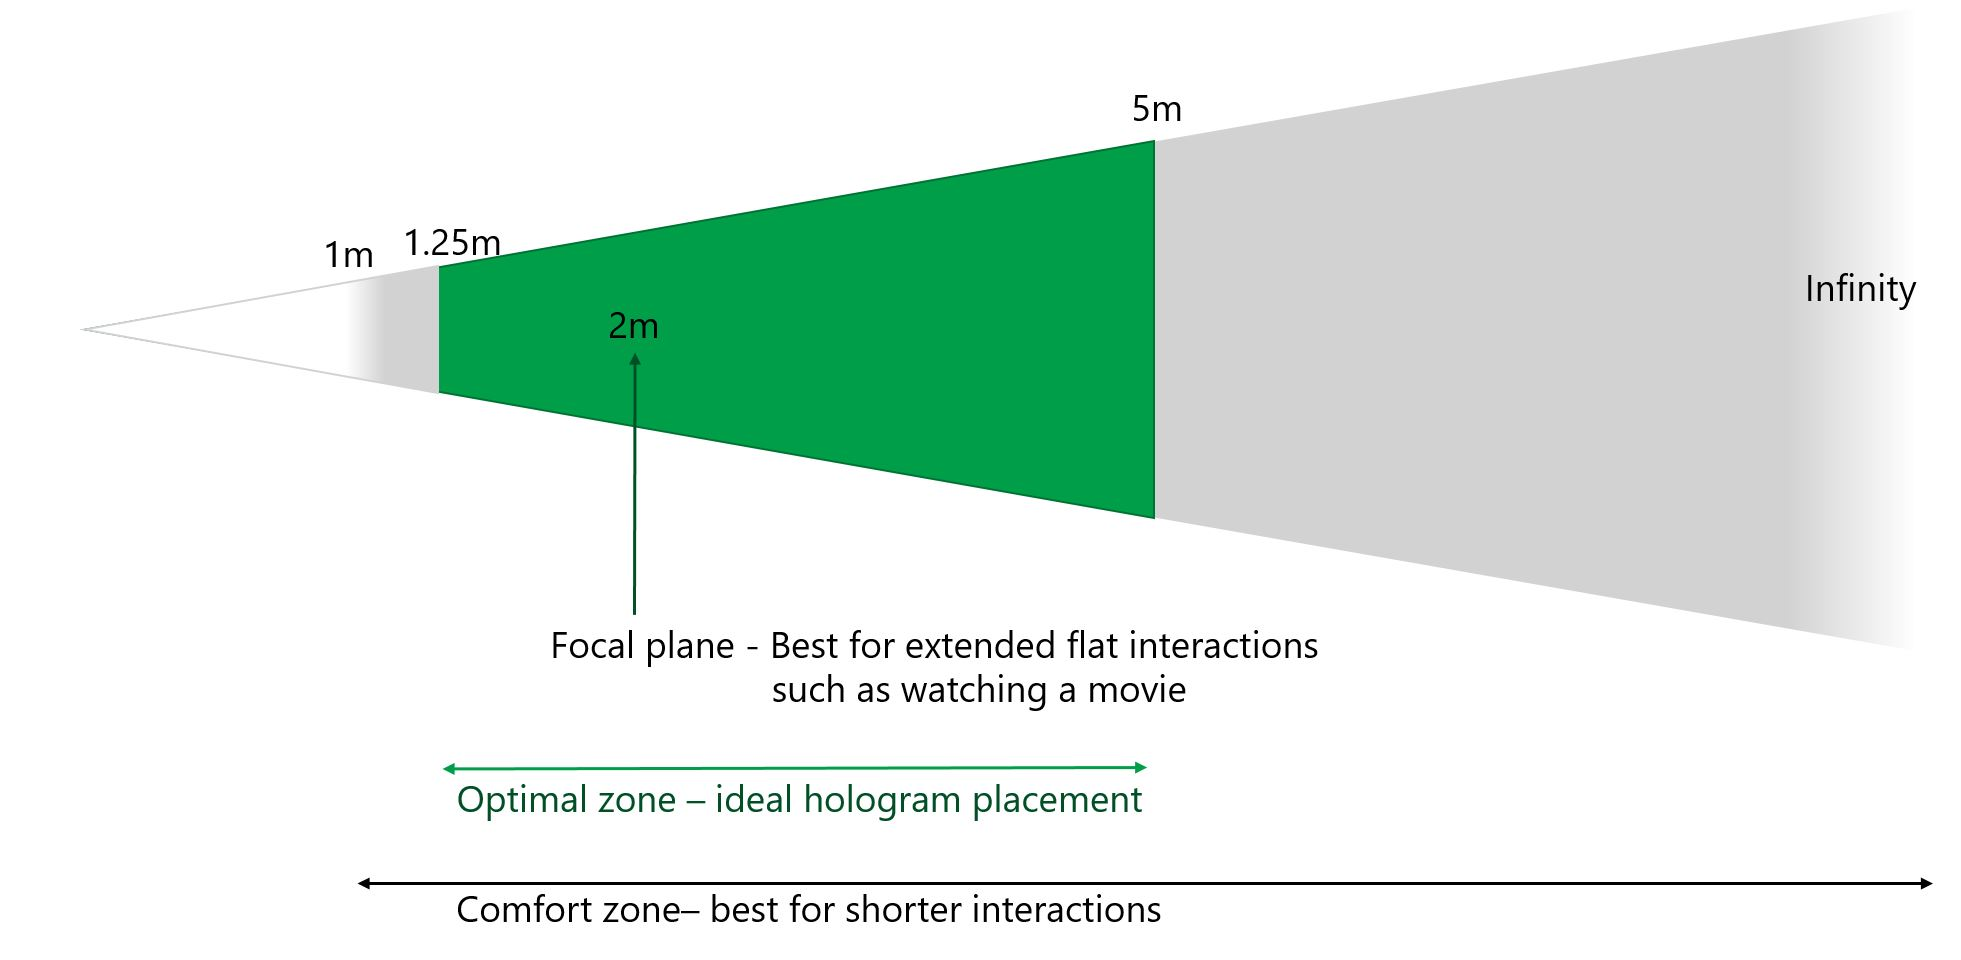
\includegraphics[width=\columnwidth]{Comfortzone}
	\caption{Optimale Distanz für die Platzierung von Hologrammen. Abbildung aus \cite{Stability}.}
\end{figure}

Die Umgebungs- und Objekterkennung funktioniert in einem 70 Grad Kegel mit einem Minimalabstand von 0,8 und einen Maximalabstand von 3,1m \cite{Design}. Abgescannte Räume und Bereiche werden abgespeichert, wiedererkannt und fortlaufend aktualisiert \cite{Mapping}. \par
Versuche während dem Projektseminar zeigten, dass die zu erkennenden Gegenstände nicht zu klein sein sollten (größer als faustgroß) und auch die Lichtverhältnisse eine Rolle spielen - z.B. beeinflussen reflektierende Oberflächen und Dunkelheit die Ergebnisse negativ. \par
Außerdem ist das Sichtfeld der HoloLens, also die Anzeige der Hologramme in der Horizontalen und Vertikalen, geringer als das Sichtfeld des Menschen. Gerade dieser Punkt wird bei der HoloLens häufig kritisiert. Microsoft gibt keine Werte an, verschiedene Messungen (siehe z.b. \cite{see}) ergaben alle ein relativ geringes Sichtfeld für die eingeblendeten Hologramme. Dieses liegt auf jeden Fall deutlich unter dem der Sensorik der HoloLens. Beispielsweise wird in \cite{fov} von einem Sichtbereich von 30x17 Grad (Breite mal Höhe) gesprochen. Auch die persönlichen Eindrücke während dem Projekt passen in diesen Rahmen. Für die Zukunft ist davon auszugehen, dass in diesem Feld Verbesserungen gemacht werden (siehe \cite{fovpatent}). \par  
Hologramme können mit der HoloLens fest verknüpft an bestimmten Punkten des Raumes platziert werden. Sie werden dabei an Wänden, Böden, Decken oder Objekten angeheftet. Dies geschieht anhand des Plans, der zuvor mit Hilfe der Umgebungserkennung erstellt wurde. Auch wenn der Nutzer sich weiterbewegt und das holographische Element aus den Augen verliert, bleibt das Hologramm an Ort und Stelle und kann bei der Rückkehr wieder betrachtet werden. Hologramme können animiert sein, bestimmte Funktionen besitzen (z.B. beim „Antippen“ per Gestensteuerung) und sich bewegen. Es gibt 2d- und 3d-Hologramme, welche man aus allen Richtungen betrachten kann. 


\section{Die HoloLens im Theaterumfeld}
Grundsätzlich können die beschriebenen Technik-Parameter der HoloLens in einer Theaterumgebung Schwierigkeiten verursachen. Insbesondere führen die Maße der Bühne und Bühnenbilder zusammen mit dem eingeschränkten Sichtfeld dazu, dass man sich in einem Abstand von der Bühne befinden muss, bei dem die automatische Erkennung des Bühnenbereichs definitiv nicht mehr funktioniert, wenn man den Überblick über ein Bühnenbild mit virtuellen Elementen bekommen möchte. Für den eingeschränkten Anwendungsrahmen des Projektes ist dies jedoch nicht unbedingt relevant. Die Theaterumgebung ist abgesehen von den Bühnenelementen relativ statisch und kann zuvor abgescannt und/oder in der HoloLens hinterlegt sein. Weiterhin sind auch die Positionsdaten der mobilen Bühnenelemente bekannt und über externe Sensoren auslesbar. Essentiell ist bei der Verwendung der HoloLens nur die Anzeige holographischer Elemente. Umgebungs- und Positionsinformationen können aus externen Quellen zugespielt werden. \par
Mit der HoloLens können Hologramme aus allen Richtungen betrachtet werden. So kann man vor der eigentlichen Fertigung des Bühnenbilds – anders als bei einem Modell - mit der Augmented Reality-Darstellung die Wirkung und Sichtbarkeit von jeder Stelle des Theaters aus überprüfen.\par
Soll die HoloLens zum Beispiel während einer Theateraufführung unterstützend für die Bedienung der Theatermaschinerie eingesetzt werden, kommt aber auch der Aspekt der Akkulaufzeit zum Tragen. Unter Last liegt die Begrenzung bei 2,5 Stunden. Eine Verlängerung dieser Zeitspanne durch extern angeschlossene Speicher ist jedoch grundsätzlich möglich. 



\section{Beschreibung des Anwendungs-Prototyps}
Für den Prototyp der Anwendung wurde die Bühne modellhaft verkleinert und auf eine einzige Laststange mit ca. 110cm Länge beschränkt. Die Applikation bildet die Laststange und eine daran befestigte Leinwand holographisch nach (siehe Abbildung \ref{Modell}). Dieses virtuelle Laststangenmodell kann mit Sprachbefehlen durch den Benutzer in Stufen in der Höhe verstellt werden. Zusätzlich zeigt die Anwendung passende Informationen dazu an: Einen Bezeichner des virtuellen Objekts (die  Laststange), die momentane Position und die Bewegungsgeschwindigkeit. Die räumliche Platzierung erfolgt über bekannte/festgelegte Koordinaten. Dafür wird ein im realen Raum liegender Markierungspunkt (QR-Code) verwendet und das virtuelle Modell daran verankert (siehe Abbildung \ref{Marker}). Es wird davon ausgegangen, dass der Abstandsvektor zwischen Markierung und Laststange bzw. den Aufhängungen aus einer externen Quelle zugespielt wird. In diesem Fall ist der Abstand konstant und im Voraus bekannt. \par

\begin{figure} 
	\centering
	
\includegraphics[width=\columnwidth]{Modell}
	\caption{Virtuelles Laststangenmodell mit Leinwand. Informationsfeld mit Bezeichner, Position und Bewegungsgeschwindigkeit rechts daneben.}
\label{Modell}
\end{figure}

\begin{figure}
	\centering
	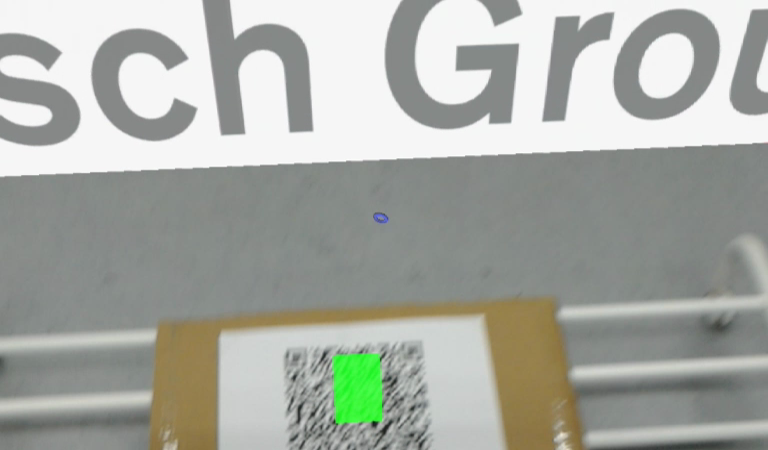
\includegraphics[width=\columnwidth]{Marker}
	\caption{QR-Code der zur Kalibrierung verwendet wird mit darüber liegender virtueller Leinwand. Der auf dem QR-Code sitzende grüne Würfel wird zur Überprüfung der korrekten Kalibrierung und Verankerung des Modells eingeblendet.}
\label{Marker}
\end{figure}

Entwickelt wurde der Prototyp mit der Game Engine Unity for Hololens (v5.4.0f3), einem Cross-Plattform-System \cite{Unity} und Visual Studio 2015. Weiterhin verwendet das Projekt das Microsoft HoloToolkit \cite{Toolkit}, eine Sammlung von Skripten und vorgefertigten Komponenten für die Entwicklung von holographischen Applikationen mit der HoloLens. Für die Marker/QR-Code Erkennung wurde Vuforia für HoloLens (v6.1) benutzt \cite{Vuforia}.\par
Gesteuert wird das System vollständig über Sprachbefehle. Der Benutzer bekommt von der Applikation Rückmeldungen via TextToSpeech geliefert.  





\section{Fazit und Ausblick}

Die holographische Darstellung von Bühnenelementen in Verknüpfung mit der tatsächlichen Theaterbühne ist zumindest im verkleinerten Modell gelungen. Eine Vergrößerung der angezeigten Elemente und die Übertragung auf die reale Theaterbühne erscheint möglich. Dabei ist aber das relativ kleine Sichtfeld der HoloLens zu beachten. Hier ist erwähnenswert, dass die Markierungs-Erkennung nur in einem sehr geringen Abstand funktioniert. Bei den verwendeten QR-Codes mit einer Größe von 15x15cm war ein Maximalabstand von ca. 0,5-1m möglich. Vergrößert man den Marker, steigt vermutlich auch der maximal mögliche Abstand. Vorstellbar ist zum Beispiel die Kalibrierung mit Markierungen in der Nähe der jeweiligen Bühnenelemente mit einer anschließenden Gesamtbetrachtung aus der Entfernung. Die Umsetzung mit Vuforia erlaubt problemlos mehrere verschiedene Marker für unterschiedliche Objekte zu verwenden. Da die Positionsdaten der Bühnenelemente bekannt sind, ist prinzipiell aber auch eine Kalibrierung mit einem einzigen, weit entfernten Marker vorstellbar. Hier müsste aber noch die Ungenauigkeit, die bei größerem Abstand der Platzierung steigt, in der realen Theaterumgebung überprüft werden. Weiterhin wurde im Projekt bisher nicht ausprobiert, ob die HoloLens bei der Anzeige von vielen und großen holographischen Objekten irgendwann an die Grenzen ihrer Leistungsfähigkeit stößt. \par
Für die holographische Einblendung von Informationen im Umfeld realer Bühnenelemente, wie etwa Lastzüge, ist ebenfalls eine genaue Positionierung nötig. Die Schwierigkeiten und Ansatzmöglichkeiten entsprechen den beschriebenen bei anderen virtuellen Elementen. Interessant ist, dass die Informationen unabhängig von der Position und dem Winkel des Betrachters angezeigt werden können. Es besteht die Möglichkeit Hologramme immer an der Blickrichtung des Benutzers auszurichten. Das Hologramm bewegt sich dann bei Kopfbewegungen mit. Dies ist sicherlich ein großer Vorteil, wenn die Bühne aus Sicherheitsgründen nicht aus den Augen gelassen werden sollte, gleichzeitig aber Informationen abgerufen werden müssen. \par
Im weiteren Verlauf des Projektes (Sommersemester 2017) ist geplant Objektinformationen (also z.B. Position der Antriebe) über Netzwerk aus dem Steuerungssystem der Bühne (bzw. einer entsprechenden Simulation) zu empfangen und danach virtuelle Objekte anhand der Objektinformationen positionieren. Für die weitere Zukunft sollen mehrere Objekte bis zum kompletten Bühnenmodell angezeigt werden können und abschließend eine Integration mit bestehender Bühnentechnik erzielt werden.   







\bibliographystyle{alphaurl}
\bibliography{Lib}

\end{document}